\documentclass{webofc}
\usepackage[varg]{txfonts}   % Web of Conferences font



\usepackage{todonotes}
\usepackage{tikz}
\usepackage{units}
\usepackage{pgfplots}
\usepackage{listings}
\usepackage{booktabs}

\usetikzlibrary{decorations.pathreplacing, patterns}
\pgfplotsset{compat=1.12}

\graphicspath{{./images/}}

\lstset{
	columns=fullflexible,
	basicstyle=\ttfamily\footnotesize,
	stringstyle=\color{green!50!black},
	keywordstyle=\color{orange!75!black},
	commentstyle=\color{white!50!black},
	emph={GooFit,Observable,DataSet,UnbinnedDataSet,BinnedDataSet,
		Variable,FitManager,
		goofit,GaussianPdf,DalitzPlotter},
	emphstyle=\color{blue!50!black}
}


% maybe use: https://github.com/olivierverdier/python-latex-highlighting/blob/master/pythonhighlight.sty

\begin{document}
%
\title{A Python upgrade to the GooFit package for parallel fitting}

\author{
	    \firstname{Henry}
        \lastname{Schreiner}\inst{1}\fnsep\thanks{\email{henry.fredrick.schreiner@cern.ch}}
        \and
        \firstname{Himadri}
        \lastname{Pandey}\inst{1}
        \and 
        \firstname{Michael D}
        \lastname{Sokoloff}\inst{1}
        \and
        \firstname{Bradley}
        \lastname{Hittle}\inst{2}
        \and 
        \firstname{Karen}
        \lastname{Tomko}\inst{2}
        \and 
        \firstname{Christoph}
        \lastname{Hasse}\inst{3}
}        % etc.

\institute{
	University of Cincinnati
\and
	Ohio Supercomputer Center
\and
	CERN / Technische Universit\"at Dortmund (DE)
}

\abstract{%
  The GooFit highly parallel fitting package for GPUs and CPUs has been substantially upgraded in the past year. Python bindings have been added to allow simple access to the fitting configuration, setup, and execution. A Python tool to write custom GooFit code given a (compact and elegant) MINT3/AmpGen amplitude description allows the corresponding C++ code to be written quickly and correctly. New PDFs have been added. The most recent release was built on top of the December 2017 2.0 release that added easier builds, new platforms, and a more robust and efficient underlying function evaluation engine.
}
%
\maketitle
%
\section{Introduction}
\label{intro}
High Energy Physics experiments around the world are producing record amounts of data. Existing tools, such as the RooFit fitting framework, provide flexible and powerful abstractions for building distributions to fit that data with, but this power comes at a cost; this is computationally expensive, and often only runs on a single core. Modern architectures provide many cores, as well as new computing paradigms, such as GPUs, that provide significant new potential for high performance computations, but are non-trivial for physicists to use to build distributions in a familiar description style.


GooFit is a high-performance multi-thread and GPU ready framework providing a similar syntax to RooFit~\cite{lib:RooFit,lib:GooFit:main}. Some comparisons are shown in figure~\ref{fig-perf} and table~\ref{tab-zachfit}. GooFit provides composition of model pieces in the same manor as RooFit, but is powered by GPUs. It also provides ready to use models for common Probability Distribution Functions (PDFs) and quantum mechanical amplitudes, as well as specialized 3-body physics models. The GooFit 2.0 release~\cite{lib:GooFit} added a simpler build process, making it easy for users to pick up and run GooFit code, and combined work from several forks, providing more physics models, 4-body models, and more features.

\begin{figure}[h]
	\centering
	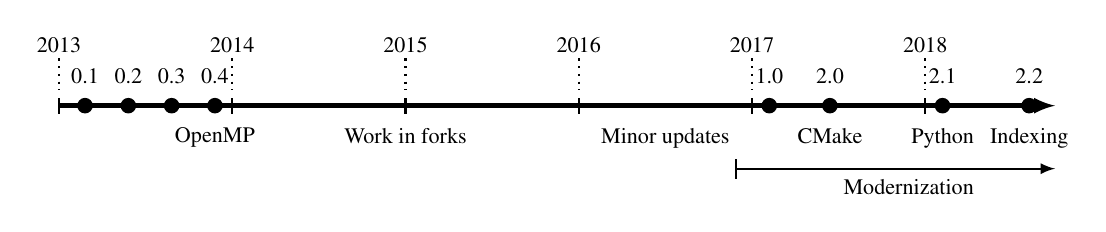
\begin{tikzpicture}[xscale=1.1,
	goonode/.style={fill=black, circle, minimum size=1.25ex, inner sep=0},
	version/.style={above=1ex, black},
	events/.style={below=1ex, black},
	every node/.style={font=\footnotesize}
	]
	\draw [-latex, ultra thick, black] (0,0) -- (11.5,0);
	\draw [|-latex, thick, black] (7.8,-.8) -- (11.5,-.8) node [midway, below, xshift=.5em] {Modernization};
	
	\foreach \x in {2013,...,2018} {
		\node at (2*\x-2*2013,0) [above=3.5ex, black] {\x};
		\draw [thick, black] (2*\x-2*2013,-.1) -- (2*\x-2*2013,.1);
		\draw [thick, dotted, black] (2*\x-2*2013,.6) -- (2*\x-2*2013,.2);
	}
	
	\node (v01) at (.3,0) [goonode] {};
	\node at (v01) [version] {0.1};
	
	\node (v02) at (.8,0) [goonode] {};
	\node at (v02) [version] {0.2};
	
	\node (v03) at (1.3,0) [goonode] {};
	\node at (v03) [version] {0.3};
	
	\node (v04) at (1.8,0) [goonode] {};
	\node at (v04) [events] {OpenMP};
	\node at (v04) [version] {0.4};
	
	\node at (4,0) [events] {Work in forks};
	
	\node (v10) at (8.2,0) [goonode] {};
	\node at (7,0) [events] {Minor updates};
	\node at (v10) [version] {1.0};
	
	\node (v20) at (8.9,0)  [goonode] {};
	\node at (v20) [events] {CMake};
	\node at (v20) [version] {2.0};
	
	\node (v21) at (10.2,0)  [goonode] {};
	\node at (v21) [events] {Python};
	\node at (v21) [version] {2.1};
	
	\node (v22) at (11.2,0)  [goonode] {};
	\node at (v22) [events] {Indexing};
	\node at (v22) [version] {2.2};
	\end{tikzpicture}%
	\caption{Timeline of GooFit development. Key points are version 2.0: New build system, C++11, and 4-body time dependent analyses support; version 2.1: Python bindings using Pybind11; and version 2.2: new indexing (and lots of Python improvements).}
	\label{fig-history}
\end{figure}

The next two releases of GooFit, given in figure~\ref{fig-history}, brings us to version 2.2, and the work contained in them will be the topic of this discussion. The most notable new change is the addition of fully functioning Python bindings, allowing users to code the composition of PDFs in a dynamic scripting language, opening up new possibilities for quick modeling and interesting interactions with other Python libraries, such as for plotting. Other changes include a new indexing system, which makes amplitudes and PDFs easier to write, and provides some small performance benefits on GPUs. A prototype for a uniform decay language, shared with other packages such as AmpGen~\cite{lib:AmpGen}, provides a powerful new frontend that can be used for user code.



\begin{figure}[h]
	\centering
	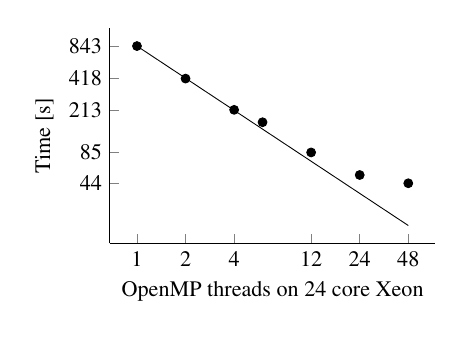
\begin{tikzpicture}[scale=.8]
	\begin{loglogaxis}[
	axis x line*=bottom,
	axis y line*=left,
	xlabel={OpenMP threads on 24 core Xeon},
	ylabel={Time [s]},
	width=6.75cm,
	height=5cm,
	log ticks with fixed point,
	xtick={1,2,4,12,24,48},
	ytick={44,85,213,418,843}
	]
	\addplot[domain=1:48] {843/x};
	\addplot [color=black, only marks] coordinates {%
		(1,843)
		(2,418)
		(4, 213)
		(6,163)
		(12, 84.98)
		(24, 52.22)
		(48,43.7)
	};
	
	\end{loglogaxis}
	\end{tikzpicture}
%
	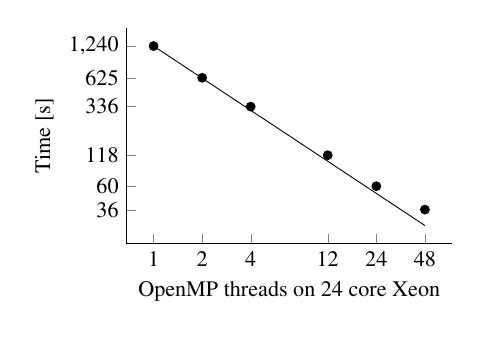
\begin{tikzpicture}[scale=.8]
	\begin{loglogaxis}[
	axis x line*=bottom,
	axis y line*=left,
	xlabel={OpenMP threads on 24 core Xeon},
	ylabel={Time [s]},
	width=6.75cm,
	height=5cm,
	log ticks with fixed point,
	xtick={1,2,4,12,24,48},
	ytick={36, 60, 118, 336, 625, 1240}
	]
	\addplot[domain=1:48] {1239.565/x};
	\addplot [color=black, only marks] coordinates {%
		(1,1239.5650)
		(2,625.0800)
		(4,335.6160)
		(12,117.7198)
		(24,60.3316)
		(48,36.4039)
	};
	
	\end{loglogaxis}
	\end{tikzpicture}
	\caption{On the left: 
		Fit from an analysis of $D^{0} \rightarrow \pi^{+}\pi^{-}\pi^0$, with 16 time-dependent amplitudes~\cite{TheBABAR:2016gom}. Original RooFit code took \unit[19,489]{s} on a single core. 40 free parameters and 100,000+ events.
		On the right:
		The ``ZachFit'': a fit to a $M (D^{*+})-M (D^0)$ measurement~\cite{paper:zachfit}. 142,576 events in an unbinned log likelyhood fit.}
	\label{fig-perf}
\end{figure}

\begin{table}[h]
	\centering
	\begin{tabular}{cccc}
		\toprule
		Number of Cores & Hardware & Pipipi0 & ZachFit \\
		\midrule
2 Cores &           Core 2 Duo & \unit[1,159]{s} & \unit[738]{s} \\
GPU &  GeForce GTX 1050 Ti & \unit[86.4]{s}& \unit[60.3]{s}   \\
GPU &            Tesla K40 & \unit[64.0]{s} & \unit[60.3]{s} \\
MPI \& GPU & Tesla K40 $\times 2$ & \unit[39.3]{s} & \unit[54.3]{s} \\
GPU &           Tesla P100 & \unit[20.3]{s}& \unit[23.5]{s} \\
\bottomrule
	\end{tabular}
\caption{GPU/CPU performance comparison. The models are the same as figure~\ref{fig-perf}. From ref.~\cite{procedings:acat2017}.}
\label{tab-zachfit}
\end{table}


\section{Python Bindings}
\label{sec-py}

Possibly the most significant new feature in the recent GooFit releases is the support for Python as a composition language. This allows simpler installation, simpler user code, faster development, easier advanced control of the fit, and interoperability with the rest of the Python ecosystem, such as for plotting.

\subsection{Building and Installing}

To install GooFit, a user now can simply use the Package Installer for Python, \texttt{pip}, to install it much like any other package. GooFit will compile from source during the install process so that it can select the maximum level of optimizations supported on your system. It will look for, and automatically use, CUDA and the GPU backend instead of the CPU backend as available. In \texttt{pip} version 10, you can simply install GooFit; older versions require you to install the SciKit-build package before installing GooFit.

This Python installer integration was provided using the SciKit-Build package, released by the developers of CMake. It adapts a CMake based build (such as GooFit) to the Python ecosystem, and is one of the reasons support for alternate build systems was added to \texttt{pip} 10. Build options, such as explicit CPU/GPU selection, can be passed through to the underlying CMake build system if needed.

In the GooFit repository, 12 of the original 13 GooFit examples have been  adapted to the new Python syntax. For many of the examples, ROOT is no longer required in the Python version, being replaced by common Python libraries.

\subsection{Syntax}

\begin{figure}[h]
	    \begin{minipage}{.51\textwidth}
		\begin{lstlisting}[language=C++]
#include <goofit/...>
using namespace GooFit;

Observable x{"x", 0, 10};
Variable mu{"mu", 1};
Variable sigma{"sigma", 1, 0, 10};
GaussianPdf gauss{"gauss", &x, &mu, &sigma};
UnbinnedDataSet ds{x};

std::mt19937 gen;
std::normal_distribution<double> d{1, 2.5};
for(size_t i=0; i<100000; i++)
	ds.addEvent(d(gen));

gauss.fitTo(&ds);

std::cout << mu << std::endl;
		\end{lstlisting}
	    \end{minipage}%
	    \begin{minipage}{.49\textwidth}
		\begin{lstlisting}[language=Python] 
from goofit import *
import numpy as np

x = Observable("x", 0, 10)
mu = Variable("mu", 1)
sigma = Variable("sigma", 1, 0, 10)
gauss = GaussianPdf("gauss", x, mu, sigma)
ds = UnbinnedDataSet(x)

data = np.random.normal(1, 2.5, (100000,1))
ds.from_matrix(data, filter=True)



gauss.fitTo(ds)

print(mu)
		\end{lstlisting}
	    \end{minipage}
	\caption{Example of GooFit 2.2 code in C++ (left) and Python (right). Some includes and main-function code have been suppressed in the C++ version for clarity. This code snippit fits a Gaussian PDF to a Gaussian distribution, and then prints the fit result for the $\mu$ parameter to the screen.}
	\label{fig-code}
\end{figure}

The syntax in the Python version of GooFit is very similar to that of the C++ version. In Python, memory is managed for the user, with Python keeping track of refcounts even when the only way to access a GooFit object is through another GooFit object.  See figure~\ref{fig-code} for a side-by-side example of C++ and Python code for GooFit.

On top of this, some ``Pythonizations'' have been added; a term popular in the Python community for writing code that looks simple and clear by utilizing Python features. An example of such a feature is setting the value of a Variable. In C++, you call  methods for setting and getting a variable's values using \texttt{setValue} and \texttt{getValue}. You can do this in Python as well, but you can also just access or assign to the \texttt{value} property on the variable. So if you want to set a variable named \lstinline|var| to 1.2, you would use either the C++ compatible expression \lstinline|val.setValue(1.2)| or the more Pythonic expression \lstinline|val.value = 1.2|. You can also use many of the built in features of Python on GooFit objects directly, such as printing, lengths, indexing, and more.

Several methods have been added to make it easy to convert events to and from Numpy arrays. The user can choose to filter out-of-range values during the conversion.There are also utilities to extract interesting quantities, evaluations, and caches from GooFit into Numpy arrays. 

\subsection{New features}

To simplify the use of GooFit from Python, several new tools were added; these tools are usually available for C++ code as well. Directly evaluating a PDF over the currently set Observable limits and binning can be done with the \texttt{evalutatePdf} method. One dimensional Monte Carlo generation on the CPU is added, as well, with the \texttt{fillMCDataSimple} method. A new tool was added called \texttt{DalitzPlotter}, which makes evaluation and simple MC generation over a 3-body amplitude model easy to do. The existing 4-body Monte Carlo generation, powered by MCBooster~\cite{lib:MCBooster}, was also improved primarily for easy Python access.

Examples were added in Python for this new functionality, using Jupyter notebooks to provide interactive visualization of 1D and Dalitz models.

\subsection{Documentation}

Documentation for GooFit has been improved and integrated with the Python bindings. Most PDFs have relevant documentation covering the mathematics that have been implemented. This is picked up by the Doxygen parser, and included in the online API documentation for the C++ code. The same documentation is also exported to the Python bindings, and gets rendered into HTML with math intact inside a Jupyter notebook if you display a PDF class. This extraction was done in CMake by selecting the Doxygen style comments, printing them out into new generated headers, and giving that to the Python bindings.

\section{The New Indexing System}
\label{sec-ind}

\begin{figure}[h]
		\centering
	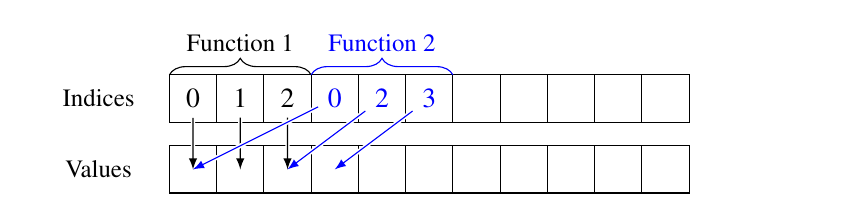
\begin{tikzpicture}[scale=.6,
	arr/.style={-latex, preaction={draw, -latex, white, ultra thick}}]
	\path[use as bounding box] (-3,-1.5) rectangle (14, 2);
	
	\foreach \x in {0,...,10} {
		\draw (\x,0) rectangle (\x+1,1);
		\draw (\x,-1.5) rectangle (\x+1,-.5);
	}
	\node at (-1.5,.5) {\small Indices};
	\node at (-1.5,-1) {\small Values};
	
	\node (a) at (0.5,.5) {0};
	\coordinate (A) at (0.5, -1);
	\draw [arr] (a) -- (A);
	
	\node (b) at (1.5,.5) {1};
	\coordinate (B) at (1.5, -1);
	\draw [arr] (b) -- (B);
	
	\node (c) at (2.5,.5) {2};
	\coordinate (C) at (2.5, -1);
	\draw [arr] (c) -- (C);
	
	\draw [decorate, decoration={brace,amplitude=6pt},xshift=0pt,yshift=0pt]
	(0,1) -- (3,1) node [black,midway,yshift=.4cm] {\small Function 1};
	
	
	\node [blue] (d) at (3.5,.5) {0};
	\draw [blue, arr] (d) -- (A);
	
	\node [blue] (e) at (4.5,.5) {2};
	\draw [blue, arr] (e) -- (C);
	
	\node [blue] (f) at (5.5,.5) {3};
	\coordinate (D) at (3.5, -1);
	\draw [blue, arr] (f) -- (D);
	
	\draw [blue, decorate, decoration={brace,amplitude=6pt},xshift=0pt,yshift=0pt]
	(3,1) -- (6,1) node [blue,midway,yshift=.4cm] {\small Function 2};
	
	\end{tikzpicture}
	\caption{The classic GooFit indexing system. Each function keeps track of a set of indices, along with the total number of indices it "owns" (not shown). GooFit then looks up the values from the given indices; this is internally referred to as GooFit's "double lookup" system. The meaning of indices are hard-coded into the function and mostly the programmers responsibility to correctly handle.}
	\label{fig-indexing-classic}
\end{figure}

\begin{figure}[h]
	\centering
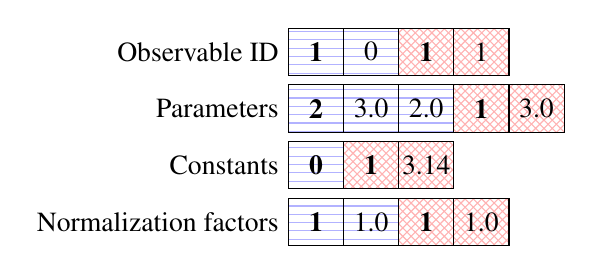
\begin{tikzpicture}[xscale=.7, yscale=.6,
first/.style={pattern=horizontal lines, pattern color=blue!30!white},
second/.style={pattern=crosshatch, pattern color=red!30!white},
ind/.style={font=\bf}]
\begin{scope}
\node at (0,0.5) [left] {Observable ID};
\draw [first, ind] (0,0) rectangle (1,1) node [midway] {1};
\draw [first] (1,0) rectangle (2,1) node [midway] {0};
\draw [second, ind] (2,0) rectangle (3,1) node [midway] {1};
\draw [second] (3,0) rectangle (4,1) node [midway] {1};
\end{scope}
\begin{scope}[yshift=-1.2cm]
\node at (0,0.5) [left] {Parameters};
\draw [first, ind] (0,0) rectangle (1,1) node [midway] {2};
\draw [first] (1,0) rectangle (2,1) node [midway] {3.0};
\draw [first] (2,0) rectangle (3,1) node [midway] {2.0};
\draw [second, ind] (3,0) rectangle (4,1) node [midway] {1};
\draw [second] (4,0) rectangle (5,1) node [midway] {3.0};
\end{scope}
\begin{scope}[yshift=-2.4cm]
\node at (0,0.5) [left] {Constants};
\draw [first, ind] (0,0) rectangle (1,1) node [midway] {0};
\draw [second, ind] (1,0) rectangle (2,1) node [midway] {1};
\draw [second] (2,0) rectangle (3,1) node [midway] {3.14};
\end{scope}
\begin{scope}[yshift=-3.6cm]
\node at (0,0.5) [left] {Normalization factors};
\draw [first, ind] (0,0) rectangle (1,1) node [midway] {1};
\draw [first] (1,0) rectangle (2,1) node [midway] {1.0};
\draw [second, ind] (2,0) rectangle (3,1) node [midway] {1};
\draw [second] (3,0) rectangle (4,1) node [midway] {1.0};
\end{scope}
\end{tikzpicture}
\caption{The new GooFit indexing system. Four arrays are stored, and instead of storing a lookup, each parameter is copied in by the underlying system as needed (potentially multiple times). This reduces the lookup cost in some cases.}
\label{fig-indexing-new}
\end{figure}

A key feature of GooFit is the indexing system; this is the system GooFit uses to allow the PDF and amplitude code to access shared values. The original system, shown in figure~\ref{fig-indexing-classic}, just stores values once, but then uses a double lookup system to find the correct index to read. The new system, shown in figure~\ref{fig-indexing-new}, uses a little preprocessing to store values in a structure that no longer requires a double lookup, saving a significant amount of time in some cases.

The indexing system redesign in GooFit 2.2 targets improved GPU performance. The indexing system in GooFit needs to track the Variables, Observables, and any constants used by any combination of PDFs. This information is packed into four separate buffers. The primary index buffer provides either a constant integer value, or contains the index into one of the three subsequent buffers which contained events, parameters, or floating-precision constants~\cite{lib:GooFit:main}. For a NVIDIA Tesla P100 GPU, 16 blocks of 32-byte sized segments specific to a thread can be cached. Two problems occur with this 32 byte memory segment that affects GPU performance. First is that if only 8 of 32 bytes are used, then the memory transaction is wasteful. Second, the segments may need to be loaded multiple times during the execution of a PDF, which is unsatisfactory for GPU performance. Using the new indexing system improves this access pattern by having memory reads behave coalesced. A side effect of the new indexing system is duplicated memory for a specific Variable or Observable. The performance improvement at the cost of this duplicating memory has a larger impact on performance by providing better memory access coherence for each PDF.

The second improvement with the indexing system provides is less complexity in developing and testing PDFs as well by providing a method for testing that indices specific in PDF construction match with the device function. Helper functions have been added allowing for registered Variables and Observables to also return the index that needs to be used within the device function. This provides a simpler mechanism for creating and debugging new PDFs by verifying indices in the device function. 

An additional change provided with the indexing update is the ParameterContainer structure which provides a consistent method for accessing all indexed values. Each device function requires a ParameterContainer reference, and each device function will need to increment the internal structure. Any additional caching techniques are hidden in this structure.

\begin{figure}[h]
	\centering
	 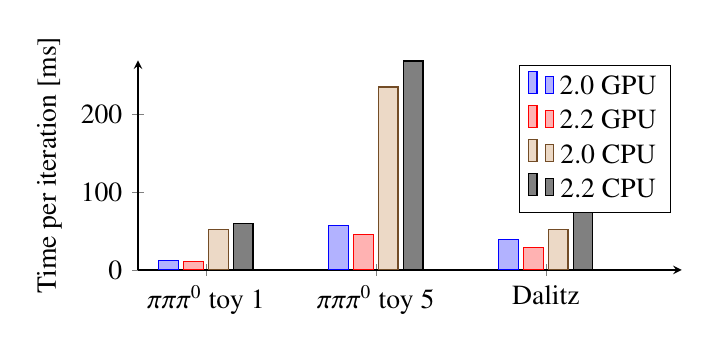
\begin{tikzpicture}
	\begin{axis}[
	ylabel={Time per iteration [ms]},
	xtick={1,2,3},
	xticklabels={$\pi\pi\pi^0$ toy 1,$\pi\pi\pi^0$ toy 5,Dalitz},
%	legend style={at={(0.5,-0.2),font=\footnotesize},
%		anchor=north,legend columns=-1},
	width=.7\textwidth,
	height=.35\textwidth,
	ybar,
	bar width=7pt,
	axis x line=bottom,
	axis y line=left,
	ymin=0,
	ymax=270,
	xmin=.6,
	xmax=3.8
	]
	% 2.0 GPU
	\addplot coordinates {
		(1,12.322)
		(2,57.259)
		(3,38.811)
	};
	% 2.2 GPU
	\addplot coordinates {
		(1,10.412)
		(2,45.358)
		(3,29.275)
	};
	\addplot coordinates {
		(1,51.99)
		(2,235.69)
		(3,52.223)
	};
	\addplot coordinates {
		(1,59.615)
		(2,269.16)
		(3,79.276)
	};
	\legend{2.0 GPU,2.2 GPU,2.0 CPU,2.2 CPU}
	\end{axis}
	\end{tikzpicture}
	\caption{Comparison of GooFit 2.0 vs GooFit 2.2 on a Dual Xeon E5-2680 with 28 cores running at 2.4 Ghz, with an NVIDIA P100 GPU. Performance gains can be seen on the GPUs when upgrading to the new indexing system in GooFit 2.2, along with slight CPU penalties.}
		\label{figure-newindexspeed}
\end{figure}

Figure \ref{figure-newindexspeed} provides a performance comparison between the old indexing system in GooFit 2.0 and the new indexing system found in GooFit 2.2 by calculating a 3-body decay. The results are captured on a Dual Xeon E5-2680 with 28 cores and an NVIDIA Tesla P100 GPU. The 3-body decay improved runtime by 32\% with GooFit 2.2 and over 9 million events.

\begin{figure}[ht]
	\centering
	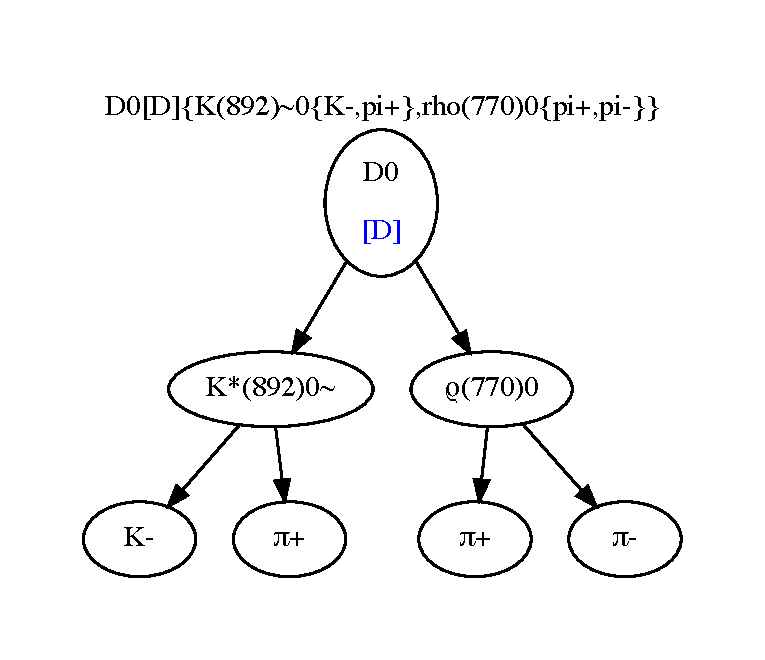
\includegraphics[width=.5\textwidth]{LineExample}
	\caption{Example of a single $D_0 \rightarrow K^{-} \pi^{+} \pi^{+} \pi^{-}$ decay using DecayLanugage's line display feature on an AmpGen line (shown at the top).}
		\label{fig-ampgen}
\end{figure}

\section{A Uniform Decay Language}
\label{sec-ampgen}

GooFit has preliminary support for decays written in the DecayLanguage syntax as implemented in AmpGen \cite{lib:AmpGen}, primarily implemented as a standalone Python package in the SciKit-HEP organization \cite{org:scikithep}.

AmpGen is a tool for compiling amplitudes for use in the LHCb event generator. It is also available as a stand-alone package apart from the LHCb framework. It builds PDFs symbolically in C++, then converts them to a C file that can be compiled into a simple library. However, it also provides a clean, powerful grammar for describing decays.

To make this language a general one that can be used across packages like GooFit, a new decay language parser was built in Python called DecayLanguage framework and released in Beta form. This implements an AmpGen compatible syntax, but is designed to produce code for other systems; the first implementation is provided, and produces C++ GooFit code. It also produces diagrams of lines in a Jupyter notebook, such as the one shown in figure~\ref{fig-ampgen}.

A comparison between the native C++ GooFit model description file and the AmpGen file for a similar decay, the  $D^0\rightarrow K^{\mp} \pi^{\pm} \pi^{\pm} \pi^{\mp}$ model \cite{paper:kthreepi}, takes 1,314 lines to describe in GooFit but only 222 lines as AmpGen grammar. The AmpGen grammar maps directly onto the physics description of the model, with one line per decay or parameter, while the GooFit code is tied up in managing memory and building C++ structures. Once converted to GooFit code by DecayLanguage, the resulting code is very similar to the handwritten code, but with helpful comments containing descriptions of the decay, and provides identical performance.



\section{Summary}
\label{sec-summary}

Three key improvements make GooFit 2.1 and 2.2 easier to use and more powerful. First, the new Python bindings allow users to access GooFit from the popular Python interpreter. This makes it easier to compose models quickly, manipulate them from scripts, and interact with the scientific Python software ecosystem.
GooFit's internal indexing system was replaced, making it simper to compose new PDFs and eliminating some common classes of mistakes for new developers. It provided a performance benefit for GPUs, and gives the GooFit core developers more flexibility for further improvements in the future.
Finally, the new DecayLanguage provides interoperability with the AmpGen package, with more packages possible in the future. This is in early stages, but provides great potential for future developments.

%For one-column wide figures use syntax of figure~\ref{fig-1}
%\begin{figure}[h]
% Use the relevant command for your figure-insertion program
% to insert the figure file.
%\centering
%\includegraphics[width=1cm,clip]{tiger}
%\caption{Please write your figure caption here}
%\label{fig-1}       % Give a unique label
%\end{figure}

%For two-column wide figures use syntax of figure~\ref{fig-2}
%\begin{figure*}
%\centering
%% Use the relevant command for your figure-insertion program
%% to insert the figure file. See example above.
%% If not, use
%\vspace*{5cm}       % Give the correct figure height in cm
%\caption{Please write your figure caption here}
%\label{fig-2}       % Give a unique label
%\end{figure*}
%
%For figure with sidecaption legend use syntax of figure
%\begin{figure}
%% Use the relevant command for your figure-insertion program
%% to insert the figure file.
%\centering
%\sidecaption
%\includegraphics[width=5cm,clip]{tiger}
%\caption{Please write your figure caption here}
%\label{fig-3}       % Give a unique label
%\end{figure}

%For tables use syntax in table~\ref{tab-1}.
%\begin{table}
%\centering
%\caption{Please write your table caption here}
%\label{tab-1}       % Give a unique label
%% For LaTeX tables you can use
%\begin{tabular}{lll}
%\hline
%first & second & third  \\\hline
%number & number & number \\
%number & number & number \\\hline
%\end{tabular}
%% Or use
%\vspace*{5cm}  % with the correct table height
%\end{table}
%
% BibTeX or Biber users please use (the style is already called in the class, ensure that the "woc.bst" style is in your local directory)
\bibliography{goofit}
%
% Non-BibTeX users please use
%
%\begin{thebibliography}{}
%%
%% and use \bibitem to create references.
%%
%
%\bibitem{GooFit}
%R Andreassen et al.
%\textit{GooFit: A library for massively parallelising maximum-likelihood fits}
%Phys.: Conf. Ser. 513 052003 (2014)
%
%\bibitem{RefJ}
%% Format for Journal Reference
%Journal Author, Journal \textbf{Volume}, page numbers (year)
%% Format for books
%\bibitem{RefB}
%Book Author, \textit{Book title} (Publisher, place, year) page numbers
%% etc
%\end{thebibliography}

% https://inspirehep.net/record/1644791 [Eur.Phys.J. C78 (2018)]

\end{document}

% end of file template.tex

<div id='footer'><table width='100%'><tr><td class='right'><a href='http://fusioninventory.org/'><span class='copyright'>FusionInventory 9.1+1.0 | copyleft <img src='/glpi/plugins/fusioninventory/pics/copyleft.png'/>  2010-2016 by FusionInventory Team</span></a></td></tr></table></div>
